\documentclass[aspectratio=169]{beamer}

% Dependency setup
\usepackage{tikz}
%

% Beamer styling setup
\usetheme{AnnArbor}
\usecolortheme{beaver}
\setbeamercolor{titlelike}{parent=structure,bg=lightgray}
%

% Spacing setup
\setlength{\parindent}{0pt} % No paragraph indenting
\setlength{\parskip}{5pt} % Set spacing between paragraphs
\frenchspacing
\newcommand{\rmspace}{\vspace{-19pt}}
%

\begin{document}
\title{Paraméteres bonyolultság}
\author{Kovács Milán, Nemkin Viktória}
\date{2021. március 16.}

\frame{\titlepage}

\frame{\frametitle{Menetrend}\tableofcontents}


\section{Motiváció}

\frame{\frametitle{Algel }}
\begin{frame}
\frametitle{Példa 1.}
\begin{itemize}
\item Sűrű vs ritka gráf.
\item Ugyanakkora az input mérete.
\item A sűrűben lassabban találunk vertex covert.
\end{itemize}
\end{frame}

\frame{\frametitle{Példa 2.}}


\section{Bar Fight Prevention problem}

\begin{frame}
\frametitle{Feladat}
Képzeljük el, hogy biztonsági őrként dolgozunk egy falusi bárban. Péntekenként nagy tömeg szokott lenni és
általában bunyóban végződik a történet... A mi feladatunk kidobni az ittas vendégeket, ami nagyon fárasztó
és nem túl mókás. Elhatározzuk, hogy megelőző intézkedéseket teszünk...

Mindenkit ismerünk a faluban és azt is tudjuk ki kivel nincs jóban, kik fognak várhatóan összeverekedni.
A tervünk tehát az, hogy csak olyan embereket engedünk be a bárba, akik jóban vannak egymással, így
elkerüljük a verekedést.

Azonban a bár menedzsmentje maximalizálni akarja a profitot, ezért azt a kikötést teszi, hogy legfeljebb
$k$ darab vendéget lehet elutasítani az ajtóban.

A feladat tehát a következő: Ismerjük a bárba bejövő emberek listáját ($n$ ember), minden emberpárra
tudjuk, hogy fognak-e verekedni ha mindkettőjüket beengedjük. Ki kell találni, hogy be lehet-e úgy
engedni az embereket, hogy legfeljebb k darab embert utasítunk el, úgy hogy bent ne törjön ki verekedés.
\end{frame}


\begin{frame}

\begin{center}
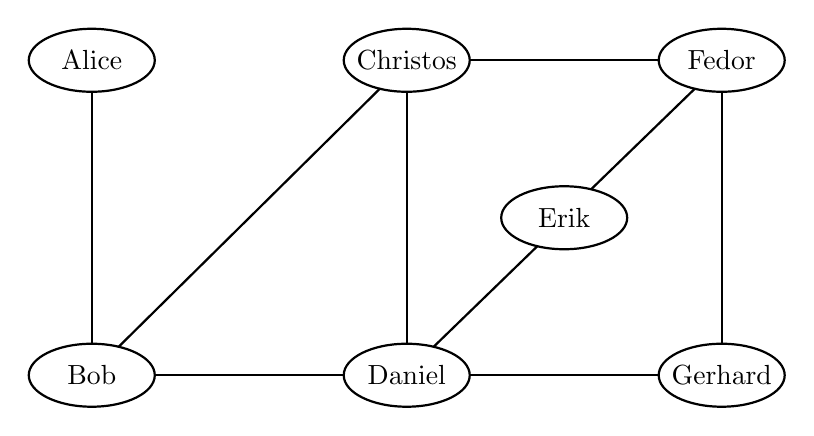
\begin{tikzpicture}[scale=2]
\draw[thick] (1,1) ellipse (0.4 and 0.2) node {Bob};
\draw[thick] (3,1) ellipse (0.4 and 0.2) node {Daniel};
\draw[thick] (5,1) ellipse (0.4 and 0.2) node {Gerhard};
\draw[thick] (4,2) ellipse (0.4 and 0.2) node {Erik};
\draw[thick] (1,3) ellipse (0.4 and 0.2) node {Alice};
\draw[thick] (3,3) ellipse (0.4 and 0.2) node {Christos};
\draw[thick] (5,3) ellipse (0.4 and 0.2) node {Fedor};

\draw[thick] (1.4,1) -- (2.6,1);
\draw[thick] (3.4,1) -- (4.6,1);
\draw[thick] (3.4,3) -- (4.6,3);

\draw[thick] (1,1.2) -- (1,2.8);
\draw[thick] (3,1.2) -- (3,2.8);
\draw[thick] (5,1.2) -- (5,2.8);

\draw[thick] (1.17,1.18) -- (2.83,2.82);
\draw[thick] (3.17,1.18) -- (3.83,1.82);
\draw[thick] (4.17,2.18) -- (4.83,2.82);

\end{tikzpicture}
\end{center}

\end{frame}

\end{document}
